\DiaryEntry{Inside Interesting Integrals, Sec. 1.8, fractional part}{2022-03-15}{Integrals}

We consider the integral (cf \cite{nahin2020inside}, Section 1.8),

\bee
I = \int_1^\infty \frac{\{x\} - \frac{1}{2}}{x} dx
\eee

where $\{x\}$ denotes the fractional part of $x$; for example, $\{0.4\} = 0, \{1.2\} = 1\}$.

The function $\{x\} - \frac{1}{2}$ (blue) and the integrand (red) are shown in the following Figure. The function $\{x\} - \frac{1}{2}$ exhibits a saw-tooth behaviour and cycles between $-1/2$ and $1/2$. The integrand is damped (due to the $x$ term in the denominator). In addition, the negative area in a length-1 interval (e.g. from $1$ to $1.5$) is bigger than the positive area in the same length-1 interval (e.g. from $1.5$ to $2$) because the negative part is damped less by the $1/x$ than the positive part. Therefore, the area under the curve must be slightly negative.

\begin{figure}[H]
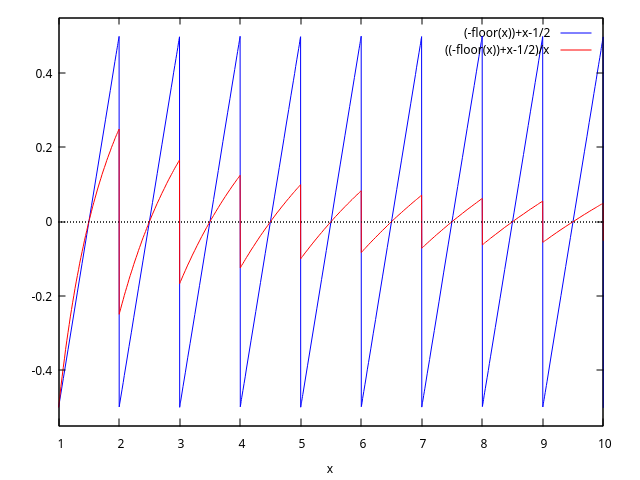
\includegraphics[scale=0.7]{images/2022-03-15_plot_1.png}
\end{figure}

The whole solution is a bit backwards; the book starts with Stirling's asymptotic formula,

\bee
n! \sim \sqrt{2\pi} n^{n+\frac{1}{2}} e^{-n}
\eee

The relative error of the approximation goes to zero for $n \rightarrow \infty$ and we have

\bee
\lim_{n \rightarrow \infty} \frac{n!}{n^{n+\frac{1}{2}} e^{-n}} = \sqrt{2\pi}
\eee

Then we start by expressing $\log n!$ as

\bee
\log n! = \log(n) + \log(n-1) + \cdots \log(2) + \log(1) = \sum_{k=2}^n \log(k)
\eee

where we have used $\log(1) = 0$ and therefore the sum starts at $k=2$. Next we observe that we can express $\log(k)$ as

\bee
\int_1^k \frac{dx}{x} = \left. \log(x) \right|_1^k = \log(k)
\eee

and using this we can rewrite our factorial expression as

\bee
\log n! = \sum_{k=2}^n \int_1^k \frac{dx}{x}
\eee

We can develop this further by splitting the integral from $1$ to $k$ into $k$ integrals having length $1$; i.e.

\bee
\int_1^k \frac{dx}{x} = \sum_{j=1}^{k-1} \int_{j}^{j+1} \frac{dx}{x}
\eee

and using this we get a double sum

\bee
\log n! = \sum_{k=2}^n \left( \sum_{j=1}^{k-1} \int_{j}^{j+1} \frac{dx}{x} \right)
\eee

The idea is to exchange the summation order; to see what we do, let's write down the sum as

\begin{align*}
  \log n! &= \int_{1}^{2} \frac{dx}{x} \\
          &+ \int_{1}^{2} \frac{dx}{x}  + \int_{2}^{3} \frac{dx}{x} \\
          &+ \int_{1}^{2} \frac{dx}{x}  + \int_{2}^{3} \frac{dx}{x} + \int_{3}^{4} \frac{dx}{x}\\
          &+ \cdots \\
          &+ \int_{1}^{2} \frac{dx}{x} + \cdots + \int_{n-1}^{n} \frac{dx}{x}
\end{align*}

where the first line corresponds to $k=2$ and the last line to $k=n$. We can see that the sum has a lower-triangular form and we can collect terms according to

\begin{align*}
  \log n! &= (n-1) \int_{1}^{2} \frac{dx}{x} + (n-2) \int_{2}^{3} \frac{dx}{x} + \cdots + \int_{n-1}^{n} \frac{dx}{x} \\
          &= \int_{1}^{2} \frac{(n-1) dx}{x} + \int_{2}^{3} \frac{(n-2) dx}{x} + \cdots + \int_{n-1}^{n} \frac{1 \cdot dx}{x}
\end{align*}

We can rewrite the integrals as

\bee
\int_{j}^{j+1} \frac{n-j}{x}dx = \int_{j}^{j+1} \frac{n - \lfloor x \rfloor}{x}dx
\eee

where $\lfloor x \rfloor$ is the floor function and we have $\lfloor x \rfloor = j$ in the (integration) interval $j \leq x  < j+1$. This allows us to combine the integrals into one as

\bee
\log n! = \int_1^n \frac{n - \lfloor x \rfloor}{x}dx
\eee

The floor function can be epxressed by the partial function as

\bee
\lfloor x \rfloor = x-  \{ x \}
\eee

and therefore the integrand can be expressed as

\bee
n - \lfloor x \rfloor = n - (x - \{ x \}) = n - x + \{ x \}
\eee

We therefore arrive at

\bee
\log n! = \int_1^n \frac{ n - x + \{ x \}  }{x}dx = \int_1^n \frac{n}{x} - 1 + \frac{\{ x \}}{x} dx
\eee

The first two expressions are easy, in the last one we sneak in a $1/(2x)$

\bee
\log n! = n \log n - (n-1) + \int_1^n \frac{1}{2x} + \frac{\{ x \} - \frac{1}{2}}{x} dx
\eee

and obtain

\bee
\log n! = n \log n - n + 1 + \frac{1}{2} \log n + \int_1^n \frac{\{ x \} - \frac{1}{2}}{x} dx
\eee

We now pull everything into the log and obtain

\bee
\log n! = \log \left( n^{n + \frac{1}{2}} e^{-n} e^{1 + \int_1^n \frac{\{ x \} - \frac{1}{2}}{x} dx} \right)
\eee

Removing the log on both sides and rearranging terms, we obtain

\bee
e^{1 + \int_1^n \frac{\{ x \} - \frac{1}{2}}{x} dx} = \frac{n!}{ n^{n + \frac{1}{2}} e^{-n}}
\eee

In the limit of large $n$, the right side becomes $\sqrt{2\pi}$ and we obtain

\bee
e^{1 + \int_1^\infty \frac{\{ x \} - \frac{1}{2}}{x} dx} = \sqrt{2\pi}
\eee

which we can solve for the integral to become

\bee
\boxed{
\int_1^\infty \frac{\{ x \} - \frac{1}{2}}{x} dx = -1 + \log \sqrt{2\pi}
}
\eee
  

The solution can be checked via Julia as follows,

\begin{verbatim}
julia> k=1:1000
1:1000

julia> sum(1 .- (2 .* k .+ 1)/2 .* log.((k.+1)./k))
-0.08097821671452388

julia> -1+log(sqrt(2*pi))
-0.08106146679532733
\end{verbatim}

\paragraph{Different Approach.} A more direct approach is to start with the integrand $\frac{\{x\} - \frac{1}{2}}{x}$ and get rid of the fraction function by splitting the integral into ``unit-integrals'' as

\bee
\int_1^\infty \frac{\{x\} - \frac{1}{2}}{x} dx = \int_1^2 \frac{\{x\} - \frac{1}{2}}{x} dx + \int_2^3 \frac{\{x\} - \frac{1}{2}}{x} dx + \cdots
\eee

Inside each integral $\int_j^{j+1}$ we then can use the fact that $\{ x \} = x-j$ and arrive at

\bee
I_N = \int_N^{N+1} \frac{\{x\} - \frac{1}{2}}{x} dx = \int_N^{N+1} \frac{x - N - \frac{1}{2}}{x} dx = \int_N^{N+1} \frac{x - \frac{2N+1}{2}}{x} dx = 1 - \frac{2N+1}{2} \log \frac{N+1}{N}
\eee

The integral $I$ is then the sum over all $I_N$ integrals but I have no idea how to combine these terms...

We can tabulate the integral $I_N$ for several value of $N$ to obtain

\begin{verbatim}
julia> [collect(N) 1 .- (2 .* N .+ 1)/2 .* log.((N .+ 1) ./ N)]
10×2 Matrix{Float64}:
  1.0  -0.0397208
  2.0  -0.0136628
  3.0  -0.00688725
  4.0  -0.00414598
  5.0  -0.00276856
  6.0  -0.00197942
  7.0  -0.00148544
  8.0  -0.0011558
  9.0  -0.000924899
 10.0  -0.000756888
\end{verbatim}

From this we can see that all integrals are negative (what was also argued in the beginningof the entry). \todo{prove this!}


%%% Local Variables:
%%% mode: latex
%%% TeX-master: "journal"
%%% End:
